\chapter{Acoustic FDTD Simulations \label{chap:acoustics}}

%\setcounter{page}{1}

\renewcommand{\thefootnote}{\fnsymbol{footnote}}
\footnotetext[2]{Lecture notes by John Schneider.  {\tt
fdtd-acoustics.tex}}

\section{Introduction}

The FDTD method employs finite-differences to approximate Ampere's and
Faraday's laws.  Ampere's and Faraday's laws are first-order
differential equations that couple the electric and magnetics fields.
As we have seen, with a judicious discretization of space and time,
the resulting equations can be solved for ``future'' fields in terms
of known past fields.  

Other physical phenomena are also described by coupled first-order
differential equations where the temporal derivative of one field is
related to the spatial derivative of another field.  Both acoustics and
elastic wave propagation are such phenomena.  Here we will consider
only acoustic propagation.  Specifically we will consider small-signal
acoustics which can be described in terms of the scalar pressure field
$P(x,y,z,t)$ and the vector velocity $\vvec(x,y,z,t)$.  The material
parameters are the speed of sound $c_a$ and the density $\rho$ (both
of which can vary as a function of position).

The governing acoustic equations in three dimensions are
\begin{eqnarray}
  \frac{\partial P}{\partial t} & = & -\rho c_a^2 \nabla\cdot\vvec,
  \label{eq:pGoverning}
  \\
  \frac{\partial \vvec}{\partial t} & = & -\frac{1}{\rho} \nabla P,
  \label{eq:vGoverning}
\end{eqnarray}
or, expanded in terms of the components,
\begin{eqnarray}
\frac{\partial P}{\partial t} & = & -\rho c_a^2
     \left(\frac{\partial v_x}{\partial x} +
           \frac{\partial v_y}{\partial y} +
           \frac{\partial v_z}{\partial z}\right) \label{eq:p-gov},\\
\frac{\partial v_x}{\partial t}
   & = & -\frac{1}{\rho} \frac{\partial P}{\partial x} \label{eq:vx-gov},\\
\frac{\partial v_y}{\partial t}
   & = & -\frac{1}{\rho} \frac{\partial P}{\partial y} \label{eq:vy-gov},\\
\frac{\partial v_z}{\partial t}
   & = & -\frac{1}{\rho} \frac{\partial P}{\partial z} \label{eq:vz-gov}.
\end{eqnarray}
Equation \refeq{eq:vGoverning} is essentially a variation of Newton's
second law, $\mathbf{F}=m\mathbf{a}$, where instead of acceleration
$\mathbf{a}$ there is the derivative of the velocity, instead of mass
$m$ there is the mass density, and instead of force $\mathbf{F}$ there
is the derivative of pressure.  Pressure is force per area and the
negative sign accounts for the fact that if pressure is building in a
particular direction that tends to cause acceleration in the opposite
direction.  Equation \refeq{eq:pGoverning} comes from an equation of
state for the material (with various approximations assumed along the
way).

Taking the divergence of \refeq{eq:vGoverning} and interchanging the
order of temporal and spatial differentiation yields 
\begin{equation}
  \frac{\partial}{\partial t}\nabla\cdot\vvec = 
  -\frac{1}{\rho} \nabla^2 P.  \label{eq:divVelocity}
\end{equation}
Taking the temporal derivative of \refeq{eq:pGoverning} and using
\refeq{eq:divVelocity} yields
\begin{equation}
  \frac{\partial^2 P}{\partial t^2} =
   -\rho c_a^2 \frac{\partial}{\partial t} \nabla\cdot\vvec =
   c_a^2 \nabla^2 P.
\end{equation}
Rearranging this yields the wave equation
\begin{equation}
     \nabla^2 P -
     \frac{1}{c_a^2} \frac{\partial^2 P}{\partial t^2} = 0.
\end{equation}
Thus the usual techniques and solutions one is familiar with from
electromagnetics carry over to acoustics.  For example, a harmonic
plane wave given by
\begin{equation}
  P(x,y,z,t) = P_0 e^{-j\boldsymbol{\beta}\cdot\mathbf{r}} e^{j\omega t}
  \label{eq:pHarmonic}
\end{equation}
is a valid solution to the governing equations where $P_0$ is a
constant and the wave vector $\boldsymbol{\beta}$ can be written
\begin{equation}
  \boldsymbol{\beta} 
  = \beta_x\unitvec{x}+\beta_y\unitvec{y}+\beta_z\unitvec{z} 
  = \beta\unitvec{\beta}=(\omega/c_a)\unitvec{\beta}.
\end{equation}

Substituting \refeq{eq:pHarmonic} into \refeq{eq:vx-gov} and assuming
$\exp(j\omega t)$ temporal dependence yields
\begin{equation}
  j \omega v_x = \frac{1}{\rho}(-j \beta_x) P.
\end{equation}
Rearranging terms gives 
\begin{equation}
  v_x = \frac{\beta_x}{\rho\omega} P.
\end{equation}
Following the same steps for the $y$ and $z$ components produces
\begin{eqnarray}
  v_y &=& \frac{\beta_y}{\rho\omega} P, \\
  v_z &=& \frac{\beta_z}{\rho\omega} P.
\end{eqnarray}
Thus the harmonic velocity is given by 
\begin{equation}
  \mathbf{v} = 
  v_x \unitvec{x} + v_y \unitvec{y} + v_z \unitvec{z}
  = \frac{1}{\rho\omega}
    (\beta_x \unitvec{x} + \beta_y \unitvec{y} + \beta_z \unitvec{z})P
  = \frac{\beta}{\rho\omega} P \unitvec{\beta}.
\end{equation}
Since the wave number, i.e., the magnitude of the wave vector, is given
by $\beta=\omega/c_a$, the ratio of the magnitude of pressure to the
velocity is given by
\begin{equation}
  \left|\frac{P}{\mathbf{v}}\right| =
  \rho c_a.
\end{equation}
The term on the right-hand side is known as the characteristic
impedance of the medium which is often written as $Z$.


\section{Governing FDTD Equations}

To obtain an FDTD algorithm for acoustic propagation, the pressure and
components of velocity are discretized in both time and space.  In
electromagnetics there were two vector fields and hence six
field-components that had to be arranged in space-time.  In acoustics
there is one scalar field and one vector field.  Thus there are only
four field-components.

To implement a 3D acoustic FDTD algorithm, a suitable arrangement of
nodes is as shown in Fig.\ \ref{fig:acousticCell}.  A pressure node is
surrounded by velocity components such that the components are
oriented along the line joining the component and the pressure node.
This should be contrasted to the arrangement of nodes in
electromagnetic grids where the components of the magnetic field
swirled around the components of the electric field, and vice versa.
In electromagnetics one is modeling coupled curl equations where the
partial derivatives are related to behavior orthogonal to the
direction of the derivative.  In acoustics, where the governing
equations involve the divergence and gradient, the partial derivatives
are associated with behavior in the direction of the derivative.

The arrangement of nodes in a 2D grid is illustrated in Fig.\
\ref{fig:acousticGridTwoD}.  This should be compared to the 2D
electromagnetic grids, i.e., Fig.\ \ref{fig:tmzGrid} for the TM$^z$
case and Fig.\ \ref{fig:tezGrid} for the TE$^z$ case.  (Because
pressure is inherently a scalar field, there are not two different
polarization associated with 2D acoustic simulations---nor is there a
notion of polarization in three dimensions.)
\begin{figure}
  \begin{center}
  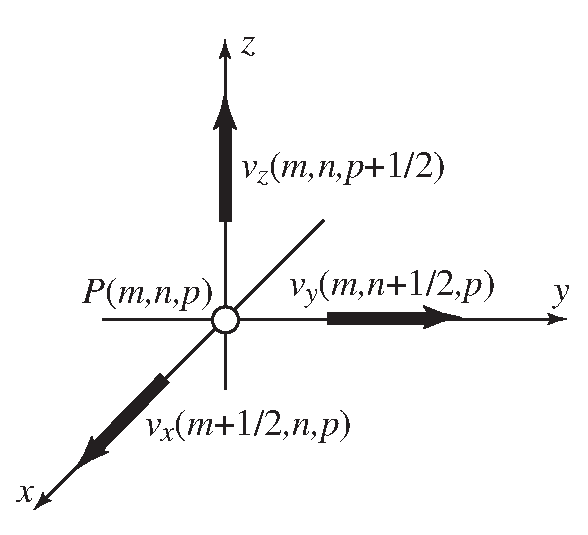
\epsfig{width=3.in,file=Figures/Fdtd-acoustics/acoustic-3d-grid.eps}
  \end{center}
  \caption{An acoustic unit cell in three dimensions showing the
  arrangement of velocity nodes relative to the pressure node with the
  same spatial indices.}
  \label{fig:acousticCell}
\end{figure}
\begin{figure}
  \begin{center}
  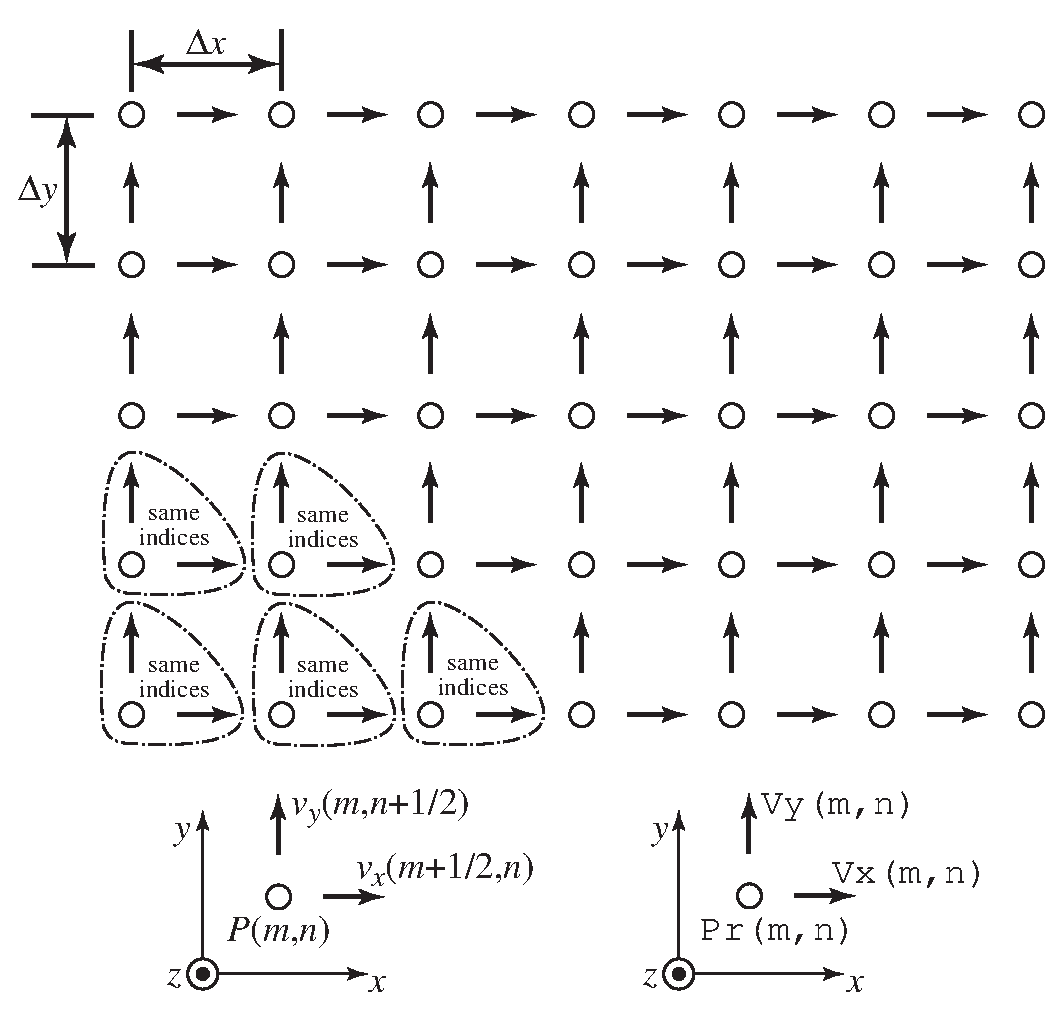
\epsfig{width=4in,file=Figures/Fdtd-acoustics/acoustic-2d-grid.eps}
  \end{center}
  \caption{The arrangement of nodes in a 2D acoustic simulation.  In
  a computer FDTD implementation the nodes shown within the dashed
  enclosures will have the same spatial indices.  This is illustrated
  by the two depictions of a unit cell at the bottom of the figure.
  The one on the left shows the nodes with the spatial offsets given
  explicitly.  The one on the right shows the corresponding node
  designations that would be used in a computer program.  (Here {\tt
  Pr} is used for the pressure array.)}
  \label{fig:acousticGridTwoD}
\end{figure}

In addition to the spatial offsets, the pressure nodes are assumed to
be offset a half temporal step from the velocity nodes (but all the
velocity components exist at the same time-step).  The following
notation will be used with an implicit understanding of spatial
offsets
\begin{eqnarray}
P(x,y,z,t) & = & P(m\Delx,n \Dely, p \Delz, q\Delt) \;=\;
 P^q[m,n,p],
 \label{eq:p-diff}\\
v_x(x,y,z,t) & = & 
  v_x\left([m+1/2]\Delx,n \Dely, p \Delz, [q+1/2]\Delt\right)
  \;=\; v_x^{q+1/2}[m,n,p], \\
v_y(x,y,z,t) & = & 
  v_y\left(m\Delx,[n+1/2] \Dely, p \Delz, [q+1/2]\Delt\right)
  \;=\; v_y^{q+1/2}[m,n,p], \\
v_z(x,y,z,t) & = & 
  v_z\left(m\Delx,n \Dely, [p+1/2] \Delz, [q+1/2]\Delt\right)
  \;=\; v_z^{q+1/2}[m,n,p]. \label{eq:vz-diff}
\end{eqnarray}
We will assume the spatial step sizes are the same, i.e., $\Delx =
\Dely = \Delz = \delta$.

Replacing the derivatives in \refeq{eq:p-gov} with finite differences
and using the discretization of \refeq{eq:p-diff}--\refeq{eq:vz-diff}
yields the following update equation:
\begin{eqnarray}
P^q[m,n,p] & = & P^{q-1}[m,n,p] -
        \rho c_a^2 \frac{\Delt}{\delta}
        \left(v_x^{q-1/2}[m,n,p]-v_x^{q-1/2}[m-1,n,p]+\mbox{}\right.
        \nonumber \\
&&                 
       	\:\,\,\,\,\quad\qquad\qquad\qquad\qquad
	\left.v_y^{q-1/2}[m,n,p]-v_y^{q-1/2}[m,n-1,p]+\mbox{}\right.
        \nonumber \\
&&                 
        \:\,\,\,\,\quad\qquad\qquad\qquad\qquad
        \left. v_z^{q-1/2}[m,n,p]-v_z^{q-1/2}[m,n,p-1]\right).
                            \label{eq:p-update}
\end{eqnarray}
The sound speed and the density can be functions of space.  Let us
assume that the density and sound speed are specified at the grid
points corresponding to the location of pressure nodes.  Additionally,
assume that the sound speed can be defined in terms of a background
sound speed $c_0$ and a relative sound speed $c_r$:
\begin{equation}
  c_a=c_rc_0.
\end{equation}
The background sound speed corresponds to the fastest speed of
propagation at any location in the grid so that $c_r\leq 1$.  The
coefficient of the spatial finite-difference in
\refeq{eq:p-update} can now be written
\begin{equation}
  \rho c_a^2 \frac{\Delt}{\delta} = 
  \rho c_r^2 c_0\frac{c_0\Delt}{\delta} = 
  \rho c_r^2 c_0 S_c 
\end{equation}
where, similar to electromagnetics, the Courant number is
$S_c=c_0\Delt/\delta$.  The explicit spatial dependence of the
density and sound speed can be emphasized by writing the coefficient
as 
\begin{equation}
  \rho[m,n,p] c_r^2[m,n,p] c_0 S_c
\end{equation}
where $\rho[m,n,p]$ is the density that exists at the same point as
the pressure node $P[m,n,p]$ and $c_r[m,n,p]$ is the relative sound
speed at this same point.  Note that the Courant number $S_c$ and the
background sound speed $c_0$ are independent of position.
Furthermore, the entire coefficient is independent of time.

The update equation for the $x$ component of velocity is obtained from
the discretized version of \refeq{eq:vx-gov} which yields
\begin{equation}
v_x^{q+1/2}[m,n,p] = v_x^{q-1/2}[m,n,p]
               -\frac{1}{\rho}\frac{\Delt}{\delta}
                \left(P^q[m+1,n,p]-P^q[m,n,p]\right)
\end{equation}
The coefficient of this equation does not contain the Courant number
but that can be obtained by multiplying and dividing by the background
sound speed
\begin{equation}
  \frac{1}{\rho}\frac{\Delt}{\delta} = 
  \frac{1}{\rho c_0}\frac{c_0\Delt}{\delta} = 
  \frac{1}{\rho c_0} S_c.
\end{equation}
We wish to define the density only at the pressure nodes.  Since
the $x$-component of the velocity is offset from the pressure a half
spatial step in the $x$ direction, what is the appropriate velocity to
use?  The answer, much as it was in the case of an interface between
two different materials in electromagnetics, is the average of the
densities to either side of the pressure node (where the notion of
``either side'' is dictated by the orientation of the velocity node).
Therefore the coefficient can be written
\begin{equation}
  \frac{1}{\left(\frac{\rho[m+1,n,p]+\rho[m,n,p]}{2}\right) c_0} S_c =
  \frac{2 S_c}{(\rho[m+1,n,p]+\rho[m,n,p]) c_0}.
\end{equation}

The update equations for the velocity components can now be written as
\begin{eqnarray}
v_x^{q+1/2}[m,n,p] &=& v_x^{q-1/2}[m,n,p] - \mbox{} \nonumber\\
               &&\hspace{-5pt}\frac{2 S_c}{(\rho[m,n,p]+\rho[m+1,n,p]) c_0}
                \left(P^q[m+1,n,p]-P^q[m,n,p]\right), \\
v_y^{q+1/2}[m,n,p] &=& v_y^{q-1/2}[m,n,p] - \mbox{} \nonumber\\
               &&\hspace{-5pt}\frac{2 S_c}{(\rho[m,n,p]+\rho[m,n+1,p]) c_0}
                \left(P^q[m,n+1,p]-P^q[m,n,p]\right), \\
v_z^{q+1/2}[m,n,p] &=& v_z^{q-1/2}[m,n,p] - \mbox{} \nonumber\\
               &&\hspace{-5pt}\frac{2 S_c}{(\rho[m,n,p]+\rho[m,n,p+1]) c_0}
                \left(P^q[m,n,p+1]-P^q[m,n,p]\right).
\end{eqnarray}

\section{Two-Dimensional Implementation}

Let us consider a 2D simulation in which the fields vary in the $x$
and $y$ directions.  The grid would be as shown in Fig.\
\ref{fig:acousticGridTwoD} and it is assumed that $\Delx = \Dely =
\delta$.  Assume the arrays {\tt pr}, {\tt vx}, and {\tt vy} hold the
pressure, $x$ component of the velocity, and the $y$ component of the
velocity, respectively.  Similar to the electromagnetic
implementation, assume the macros {\tt Pr}, {\tt Vx}, and {\tt Vy}
have been created to facilitate accessing these arrays (ref.\ Sec.\
\ref{sec:multiArrays}).  The update equations can be written
\begin{verbatim}
  Vx(m,n) = Vx(m,n) - Cvxp(m,n)*(Pr(m+1,n) - Pr(m,n));
  Vy(m,n) = Vy(m,n) - Cvyp(m,n)*(Pr(m,n+1) - Pr(m,n));
  Pr(m,n) = Pr(m,n) - Cprv(m,n)*((Vx(m,n) - Vx(m-1,n)) 
                               + (Vy(m,n) - Vy(m,n-1)));
\end{verbatim}
where the coefficient arrays are given by
\begin{eqnarray}
  \cvxp(m,n) &=&
    \left.\frac{1}{\rho c_0} S_c\right|_{(m+1/2)\delta,n\delta} =
    \frac{2 S_c}{(\rho[m+1,n]+\rho[m,n]) c_0}, \\
  \cvyp(m,n) &=&
    \left.\frac{1}{\rho c_0} S_c\right|_{m\delta,(n+1/2)\delta} =
    \frac{2 S_c}{(\rho[m,n]+\rho[m,n+1]) c_0}, \\
  \cprv(m,n) &=& \rho[m,n] c_r^2[m,n] c_0 S_c.
\end{eqnarray}

These update equations are little different from those for the TM$^z$
case.  Referring to Sec.\ \ref{sec:tmzPolarization} for lossless
materials, the TM$^z$ update equations are
\begin{verbatim}
  Hy(m,n) = Hy(m,n) + Chye(m,n)*(Ez(m+1,n) - Ez(m,n));
  Hx(m,n) = Hx(m,n) - Chxe(m,n)*(Ez(m,n+1) - Ez(m,n));
  Ez(m,n) = Ez(m,n) + Cezh(m,n)*((Hy(m,n) - Hy(m-1,n))
                                -(Hx(m,n) - Hx(m,n-1)));
\end{verbatim}
There is a one-to-one mapping between these sets of equations.
One can equate values as follows
\begin{eqnarray}
  v_x &\Leftrightarrow& -H_y, \\
  v_y &\Leftrightarrow& H_x, \\
  P   &\Leftrightarrow& E_z,\\
  \cvxp &\Leftrightarrow& \chye, \\
  \cvyp &\Leftrightarrow& \chxe, \\
  \cprv &\Leftrightarrow& \cezh.
\end{eqnarray}
Thus, converting 2D programs that were written to model
electromagnetic field propagation to ones that can model acoustic
propagation is surprisingly straightforward.  Essentially, all one has
to do is change some labels and a few signs.

For TE$^z$ simulations, the updated equations for a lossless medium
were
\begin{verbatim}
  Hz(m,n) = Hz(m,n) +
            Chze(m,n)*((Ex(m,n+1)-Ex(m,n))-(Ey(m+1,n)-Ey(m,n)));
  Ex(m,n) = Ex(m,n) + Cexh(m,n)*(Hz(m,n)-Hz(m,n-1));
  Ey(m,n) = Ey(m,n) - Ceyh(m,n)*(Hz(m,n)-Hz(m-1,n));
\end{verbatim}
In this case the conversion from the electromagnetic equations to the
acoustic equations can be accomplished with the following mapping
\begin{eqnarray}
  v_x &\Leftrightarrow& E_y, \\
  v_y &\Leftrightarrow& -E_x, \\
  P   &\Leftrightarrow& H_z,\\
  \cvxp &\Leftrightarrow& \ceyh, \\
  \cvyp &\Leftrightarrow& \cexh, \\
  \cprv &\Leftrightarrow& \chze.
\end{eqnarray}

For three dimensions 3D acoustic code is arguably simpler than the
electromagnetic case since there are not two vector fields.  However
porting 3D electromagnetic algorithms to the acoustic case is not as
trivial as in two dimensions.
